\chapter{Eletromagnetismo covariante}\label{ch:b3:covariant-electromagnetism}

Um fio de cobre conduz dez ampères. Seus elétrons derivam a um décimo
de milímetro por segundo --- mais devagar que um caracol --- e o fio é
eletricamente neutro com precisão fantástica. Ainda assim, uma carga
que se move ao lado dele sente uma atração mensurável. Vista do
referencial próprio dessa carga, a explicação ``magnética'' evapora: a
carga está em repouso, e uma carga em repouso não sente força magnética
alguma. O que a puxa, nesse referencial, é um campo \emph{elétrico} ---
conjurado pela própria relatividade, porque a \omterm{prop:b3:relativistic-kinematics:contraction}{contração dos
comprimentos} desequilibra, em uma parte em
$10^{24}$, as duas correntes de carga do fio. O magnetismo é a
eletricidade vista de um assento em movimento. Este capítulo reescreve
o eletromagnetismo do volume do segundo ano na linguagem dos três
capítulos anteriores: \omterm{def:b3:covariant-electromagnetism:fourvector}{quadrivetores} para a carga e o potencial, um
único tensor antissimétrico que mantém $\vect E$ e $\vect B$ juntos, e
as quatro equações de Maxwell reduzidas a duas linhas que se leem do
mesmo modo em todo \omterm{thm:b3:relativistic-kinematics:postulates}{referencial inercial}. Além da elegância, o proveito
é física em funcionamento: como os campos se transformam, por que o
campo de uma carga rápida se achata num disco e por que a luz de um
elétron relativístico varre para a frente como um farol --- o princípio
das fontes de luz síncrotron que hoje radiografam proteínas e baterias.

\section{Quadrivetores para a carga e a corrente}

\begin{definition}[Quadrivetores]\label{def:b3:covariant-electromagnetism:fourvector}
\index{quadrivetor}
Um \emph{quadrivetor} é uma quádrupla $a^\mu = (a^0, \vect a)$, $\mu =
0, 1, 2, 3$, cujas componentes se misturam sob um impulso de Lorentz
exatamente como $(ct,
\vect r)$ se misturam:
\[
a'^0 = \gamma(a^0 - \beta a^1) , \qquad
a'^1 = \gamma(a^1 - \beta a^0) , \qquad
a'^{2,3} = a^{2,3}
\]
para um impulso a $\beta c$ ao longo de $x$. Dois quadrivetores
quaisquer dão o produto escalar invariante
$a\cdot b = a^0b^0 - \vect a\cdot\vect b$, o mesmo número em todo
referencial --- o padrão por trás de $c^2t^2 - x^2$ e de
$E^2 - p^2c^2$. A posição $(ct, \vect r)$ e o \omterm{def:b3:relativistic-dynamics:four-momentum}{quadrimomento}
$(E/c, \vect p)$ são os dois que já temos; o eletromagnetismo fornece
agora mais três: corrente, potencial e vetor de onda.
\end{definition}

\begin{proposition}[A quadricorrente e a conservação da carga]\label{prop:b3:covariant-electromagnetism:fourcurrent}
\index{quadricorrente}
A densidade de carga $\rho$ e a densidade de corrente $\vect\jmath$
formam a quadricorrente
\[
J^\mu = (\rho c,\ \vect\jmath\,) :
\]
uma nuvem de carga de densidade própria $\rho_0$ que se move com
$\vect u$ tem $J^\mu = \rho_0\gamma_u(c, \vect u)$ --- a densidade
cresce por $\gamma_u$ porque o volume da nuvem se contrai, ao passo que
a própria carga é invariante (um fato experimental decisivo: átomos com
elétrons internos velozes permanecem exatamente neutros). A conservação
da carga é o enunciado invariante
\[
\frac{\partial(\rho c)}{\partial(ct)} +
\operatorname{div}\vect\jmath = 0 ,
\]
a equação da continuidade do volume do segundo ano, agora visivelmente
a mesma lei para todos os observadores.
\end{proposition}

\begin{proof}[Demonstração parcial]
A nuvem em movimento: uma caixa de volume próprio $V_0$ contém a carga
$\rho_0
V_0$; no laboratório a caixa está contraída a $V_0/\gamma_u$, logo $\rho =
\gamma_u\rho_0$, e $\vect\jmath = \rho\vect u$ pela definição
de densidade de corrente. Que $(\rho c, \vect\jmath)$ se transforme
então como \omterm{def:b3:covariant-electromagnetism:fourvector}{quadrivetor} decorre de ele ser igual a $\rho_0/c$ vezes a
quadrivelocidade $\gamma_u(c, \vect u)$, ela própria um \omterm{def:b3:covariant-electromagnetism:fourvector}{quadrivetor} por
construção. A invariância da carga é um dado experimental.
\end{proof}

\section{Um só tensor para os dois campos}

\begin{definition}[Quadripotencial e tensor do campo]\label{def:b3:covariant-electromagnetism:tensor}
\index{quadripotencial}\index{tensor do campo}
Os potenciais do volume do segundo ano se reúnem no quadripotencial
\[
A^\mu = \Big(\frac{V}{c},\ \vect A\Big) ,
\]
e os campos mensuráveis $\vect E = -\vect\nabla V -
\partial_t\vect A$, $\vect B = \operatorname{\vect{curl}}\vect A$ são
as seis componentes independentes de um único arranjo antissimétrico, o
\emph{tensor do campo eletromagnético}
\[
F^{\mu\nu} =
\begin{pmatrix}
0 & -E_x/c & -E_y/c & -E_z/c\\
E_x/c & 0 & -B_z & B_y\\
E_y/c & B_z & 0 & -B_x\\
E_z/c & -B_y & B_x & 0
\end{pmatrix} .
\]
$\vect E$ e $\vect B$ não são dois campos, mas seis faces de um mesmo
objeto; qual delas um observador chama de ``elétrica'' depende do
movimento do observador.
\end{definition}

\begin{theorem}[Maxwell, de forma covariante]\label{thm:b3:covariant-electromagnetism:maxwell}
\index{equações de Maxwell!forma covariante}
As quatro equações de Maxwell do volume do segundo ano são a forma em
componentes de dois enunciados independentes do referencial: o par com
fontes (Gauss e Ampère--Maxwell) é
\[
\sum_\mu \partial_\mu F^{\mu\nu} = \mu_0\,J^\nu ,
\]
e o par sem fontes (ausência de monopolos, Faraday) é a identidade que
garante que $F$ deriva de um \omterm{def:b3:covariant-electromagnetism:tensor}{quadripotencial}. A força de Lorentz é
$\dd p^\mu/\dd\tau = qF^{\mu\nu}u_\nu$ --- a lei da força, magnética
inclusa, numa só linha. Como os dois lados de cada equação se
transformam do mesmo modo, \emph{a teoria de Maxwell não precisa de
correção alguma para ser relativística}: foi a primeira peça acabada da
relatividade, nascida em 1865.
\end{theorem}

\begin{proof}[Demonstração parcial]
Expanda a componente $\nu = 0$: $\sum_i\partial_i(E_i/c) =
\mu_0\rho c$, isto é, $\operatorname{div}\vect E = \rho/\varepsilon_0$
(usando $c^2 = 1/\mu_0\varepsilon_0$). A componente $\nu = 1$ reúne
$-\partial_t(E_x/c^2) + (\partial_yB_z - \partial_zB_y)
= \mu_0 j_x$: a componente $x$ de Ampère--Maxwell. As demais
componentes repetem o padrão; o par sem fontes é a igualdade das
derivadas segundas cruzadas de $A^\mu$ (verificada no
\cref{exo:b3:covariant-electromagnetism:3}). Que $F^{\mu\nu}$ se
transforme como um tensor (de dois índices) --- cada índice como um
\omterm{def:b3:covariant-electromagnetism:fourvector}{quadrivetor} --- é admitido; suas consequências são a próxima
proposição.
\end{proof}

\section{Como os campos se transformam}

\begin{proposition}[Transformação dos campos]\label{prop:b3:covariant-electromagnetism:transform}
\index{transformação dos campos}
Para um impulso de velocidade $\vect v = v\,\vect e_x$: as componentes
\emph{ao longo} do movimento ficam intactas, as transversais se
misturam,
\[
E'_x = E_x , \qquad
E'_y = \gamma(E_y - vB_z) , \qquad
E'_z = \gamma(E_z + vB_y) ,
\]
\[
B'_x = B_x , \qquad
B'_y = \gamma\Big(B_y + \frac{v}{c^2}E_z\Big) , \qquad
B'_z = \gamma\Big(B_z - \frac{v}{c^2}E_y\Big) .
\]
De modo compacto, transversalmente ao impulso: $\vect E' = \gamma(\vect E +
\vect v\wedge\vect B)_\perp$ e $\vect B' = \gamma(\vect B - \vect
v\wedge\vect E/c^2)_\perp$. Um $\vect B$ puro num referencial é $\vect
E$ e $\vect B$ em outro: os campos são um único fenômeno.
\end{proposition}
\admitted

\begin{example}[Magnetismo a partir de um fio neutro]\label{ex:b3:covariant-electromagnetism:wire}
Um fio neutro conduz corrente: rede positiva em repouso, elétrons em
deriva. Para uma carga de prova que se move ao lado, passe ao
referencial dela: as duas correntes de carga se contraem de modo
\emph{diferente} (têm velocidades diferentes), o fio adquire a carga
linear líquida $\lambda' =
-\gamma vI/c^2$, e seu campo elétrico radial puxa a carga exatamente
com a força que o laboratório chamava de $q\vect v\wedge\vect B$. O
magnetismo é a aparência do termo de segunda ordem $v u/c^2$ da
relatividade quando $10^{28}$ cargas elementares por metro conspiram:
cada efeito é fantasticamente pequeno, mas o fio é neutro com precisão
ainda maior, de modo que o desequilíbrio minúsculo é a história inteira
(\cref{pb:b3:covariant-electromagnetism:1}).
\end{example}

\begin{omfigure}
\begin{tikzpicture}[font=\small, >=Stealth]
  % lab frame
  \begin{scope}
    \draw[thick, fill=omExo!10] (-0.2,0) rectangle (5.4,0.75);
    \foreach \x in {0.3,1.3,2.3,3.3,4.3} \node[omThm] at (\x,0.52) {$\oplus$};
    \foreach \x in {0.8,1.8,2.8,3.8,4.8} {\node[omDef] at (\x,0.22) {$\ominus$};
      \draw[->, omDef] (\x+0.16,0.22) -- (\x+0.42,0.22);}
    \fill[omProp] (2.6,-1.15) circle (2.6pt);
    \draw[->, omProp, thick] (2.75,-1.15) -- (3.55,-1.15);
    \node[anchor=west] at (3.65,-1.15) {$q$, velocidade $v$};
    \draw[->, very thick] (2.6,-0.95) -- (2.6,-0.35);
    \node[anchor=west, font=\footnotesize] at (2.7,-0.62) {$q\vect v\wedge\vect B$};
    \node at (2.6,1.35) {laboratório: fio neutro, força magnética};
  \end{scope}
  % charge frame
  \begin{scope}[xshift=7.8cm]
    \draw[thick, fill=omExo!10] (-0.2,0) rectangle (5.4,0.75);
    \foreach \x in {0.25,1.15,2.05,2.95,3.85,4.75} {\node[omThm] at (\x,0.52) {$\oplus$};
      \draw[->, omThm] (\x-0.14,0.72) -- (\x-0.4,0.72);}
    \foreach \x in {0.7,1.9,3.1,4.3} \node[omDef] at (\x,0.22) {$\ominus$};
    \fill[omProp] (2.6,-1.15) circle (2.6pt);
    \node[anchor=west] at (2.75,-1.35) {$q$ em repouso};
    \draw[->, very thick] (2.6,-0.95) -- (2.6,-0.35);
    \node[anchor=west, font=\footnotesize] at (2.7,-0.62) {$q\vect E'$};
    \node at (2.6,1.35) {referencial da carga: fio carregado, força elétrica};
  \end{scope}
\end{tikzpicture}

{\small Uma força, duas contabilidades. Laboratório: a corrente do fio
neutro cria $\vect B$, e a carga em movimento sente
$q\vect v\wedge\vect B$. Referencial da carga: a rede positiva agora se
move e se contrai, e os elétrons (mais lentos ali) se espalham; o fio
tem carga líquida e é o $\vect E'$ dele que puxa. Mesmo experimento,
mesmo desfecho.}
\end{omfigure}

\begin{example}[O campo achatado de uma carga rápida]\label{ex:b3:covariant-electromagnetism:pancake}
Transforme o campo de Coulomb de uma carga para o referencial em que
ela se move com $\gamma \gg 1$: o campo longitudinal não muda, enquanto
o transversal é multiplicado por $\gamma$. O campo, antes esférico,
achata-se num disco de abertura angular $\sim 1/\gamma$ em torno do
plano que passa pela carga --- acompanhado, transversalmente ao
movimento, por um anel magnético $B' = vE'/c^2$. Para um observador
parado, a passagem de um próton do LHC ($\gamma \approx 7000$) é uma
bofetada sub-picossegundo de $\vect E$ e $\vect B$ quase cruzados:
quase um pulso de luz --- a razão de os feixes rápidos falarem com a
matéria do jeito que os fótons falam.
\end{example}

\begin{omfigure}
\begin{tikzpicture}[font=\small, >=Stealth]
  % static charge
  \begin{scope}
    \fill[omThm] (0,0) circle (2.6pt);
    \foreach \a in {0,30,...,330} \draw[->, omDef] (\a:0.25) -- (\a:1.75);
    \node at (0,-2.5) {em repouso: campo de Coulomb isotrópico};
  \end{scope}
  % moving charge
  \begin{scope}[xshift=8.0cm]
    \fill[omThm] (0,0) circle (2.6pt);
    \draw[->, very thick] (0.3,-2.1) -- (1.5,-2.1) node[right] {$v \approx c$};
    \foreach \a/\l in {90/1.95, 75/1.5, 105/1.5, 60/0.85, 120/0.85,
                       270/1.95, 255/1.5, 285/1.5, 240/0.85, 300/0.85,
                       0/0.35, 180/0.35, 30/0.45, 150/0.45, 210/0.45, 330/0.45}
      \draw[->, omDef] (\a:0.25) -- (\a:\l);
    \node at (0,-2.5) {};
    \node at (0.3,-2.65) {};
    \node at (0,-2.9) {};
  \end{scope}
  \node at (8.0,-2.5) {em movimento: campo achatado em $\sim 1/\gamma$};
\end{tikzpicture}

{\small O campo elétrico de uma carga pontual, em repouso e a alta
velocidade: o impulso de Lorentz multiplica as componentes transversais
por $\gamma$ e deixa as longitudinais intactas, espremendo o campo num
disco perpendicular ao movimento.}
\end{omfigure}

\section{Invariantes, luz e o efeito farol}

\begin{proposition}[Os dois invariantes do campo]\label{prop:b3:covariant-electromagnetism:invariants}
\index{invariantes do campo}
A partir de $F^{\mu\nu}$ podem-se construir exatamente dois escalares
independentes:
\[
E^2 - c^2B^2
\qquad\text{e}\qquad
\vect E\cdot\vect B ,
\]
os mesmos em todo \omterm{thm:b3:relativistic-kinematics:postulates}{referencial inercial}. Consequências: se $E > cB$ em
algum lugar (com $\vect E\cdot\vect B = 0$), algum referencial vê ali
um campo puramente elétrico; se $E < cB$, algum referencial o vê
puramente magnético; e uma onda plana de luz, com $E = cB$ e
$\vect E\perp\vect B$, tem \emph{os dois} invariantes nulos --- é luz
em todo referencial: nenhum impulso pode transformá-la num campo
estático, apenas desviá-la para o vermelho. Não se pode alcançar uma
onda de luz; a pergunta de adolescente de Einstein se responde a si
mesma em dois invariantes.
\end{proposition}

\begin{proof}[Demonstração parcial]
Verifique a invariância sob o impulso padrão por substituição direta da
\cref{prop:b3:covariant-electromagnetism:transform}
(\cref{exo:b3:covariant-electromagnetism:6}); que não exista um
terceiro invariante independente é admitido. Para a onda: $E = cB$ e a
ortogonalidade anulam os dois; um referencial com campo estático
exigiria um invariante não nulo.
\end{proof}

\begin{proposition}[Quadrivetor de onda, Doppler e aberração]\label{prop:b3:covariant-electromagnetism:wavevector}
\index{aberração}\index{efeito farol}
A frequência e a direção de uma onda plana formam o \omterm{def:b3:covariant-electromagnetism:fourvector}{quadrivetor} nulo
$k^\mu = (\omega/c, \vect k)$, $\|\vect k\| = \omega/c$. Transformá-lo
dá de uma vez a fórmula relativística do efeito Doppler do
\cref{ch:b3:relativistic-kinematics} e a \emph{aberração} das
direções:
\[
\cos\theta' = \frac{\cos\theta - \beta}{1 - \beta\cos\theta} .
\]
Lida ao contrário, uma fonte que irradia isotropicamente em seu
referencial de repouso concentra, no laboratório, metade de sua luz no
cone dianteiro $\theta
\lesssim 1/\gamma$: é o \emph{\omterm{prop:b3:covariant-electromagnetism:wavevector}{efeito farol}}. Um elétron que gira a
$\gamma \sim 10^4$ num anel de armazenamento varre um holofote de
raios X de $\qty{0.1}{mrad}$ ao redor do anel --- a luz síncrotron que
abastece as linhas de cristalografia de proteínas.
\end{proposition}

\begin{proof}[Demonstração parcial]
A fase $\omega t - \vect k\cdot\vect r = k^\mu x_\mu$ conta as cristas
de onda que passam por eventos --- um invariante --- de modo que
$k^\mu$ tem de se transformar como \omterm{def:b3:covariant-electromagnetism:fourvector}{quadrivetor}. Aplique o impulso a
$(\omega/c, k\cos\theta,
k\sin\theta, 0)$: a componente temporal dá o efeito Doppler, e a razão
das componentes espaciais dá a fórmula da aberração. Impondo $\theta' =
90^\circ$ (o raio lateral no referencial da fonte):
$\cos\theta =
\beta$, isto é, $\theta \approx 1/\gamma$ para $\gamma \gg 1$ ---
metade da esfera se dobra dentro do cone dianteiro.
\end{proof}

\begin{omfigure}
\begin{tikzpicture}[font=\small, >=Stealth]
  % isotropic source
  \begin{scope}
    \fill[omThm] (0,0) circle (2.4pt);
    \foreach \a in {0,45,...,315} \draw[->, omExo] (\a:0.3) -- (\a:1.5);
    \node at (0,-2.2) {referencial de repouso: isotrópico};
  \end{scope}
  % beamed
  \begin{scope}[xshift=7.6cm]
    \fill[omThm] (0,0) circle (2.4pt);
    \draw[->, thick] (-1.9,0) -- (-0.6,0);
    \node at (-2.35,0) {$v$};
    \draw[->, omExo] (0.3,0.06) -- (2.6,0.55);
    \draw[->, omExo] (0.3,-0.06) -- (2.6,-0.55);
    \draw[->, omExo, very thick] (0.3,0) -- (2.9,0);
    \draw[->, omExo] (0.25,0.16) -- (1.5,1.0);
    \draw[->, omExo] (0.25,-0.16) -- (1.5,-1.0);
    \draw[->, omExo] (-0.1,0.28) -- (-0.5,1.0);
    \draw[->, omExo] (-0.1,-0.28) -- (-0.5,-1.0);
    \draw[dashed] (0,0) -- (3.1,0.85);
    \draw[dashed] (0,0) -- (3.1,-0.85);
    \node[anchor=west, font=\footnotesize] at (3.0,0.5) {$\sim 1/\gamma$};
    \node at (0.9,-2.2) {laboratório: um farol para a frente};
  \end{scope}
\end{tikzpicture}

{\small A aberração dobra a radiação de uma fonte rápida num cone
dianteiro de semiabertura $\sim 1/\gamma$: o \omterm{prop:b3:covariant-electromagnetism:wavevector}{efeito farol}, e o
princípio de funcionamento das fontes de luz síncrotron.}
\end{omfigure}

\begin{method}[Trabalhar de modo covariante]\label{met:b3:covariant-electromagnetism:method}
(1) Identifique os \omterm{def:b3:covariant-electromagnetism:fourvector}{quadrivetores} em jogo ($x^\mu$, $P^\mu$, $J^\mu$,
$A^\mu$, $k^\mu$) e prefira seus produtos invariantes às componentes.
(2) Para transformar campos, separe as componentes ao longo e
transversalmente ao impulso e aplique a
\cref{prop:b3:covariant-electromagnetism:transform}. (3) Verifique os
dois invariantes antes e depois --- o detector de erros mais rápido do
assunto. (4) Quando um problema magnético parecer misterioso, viaje com
a carga: no referencial dela só $\vect E'$ age. (5) Confie em Maxwell:
as equações nunca precisam de ``correções'' relativísticas, apenas de
uma leitura relativística.
\end{method}

\begin{omfigure}
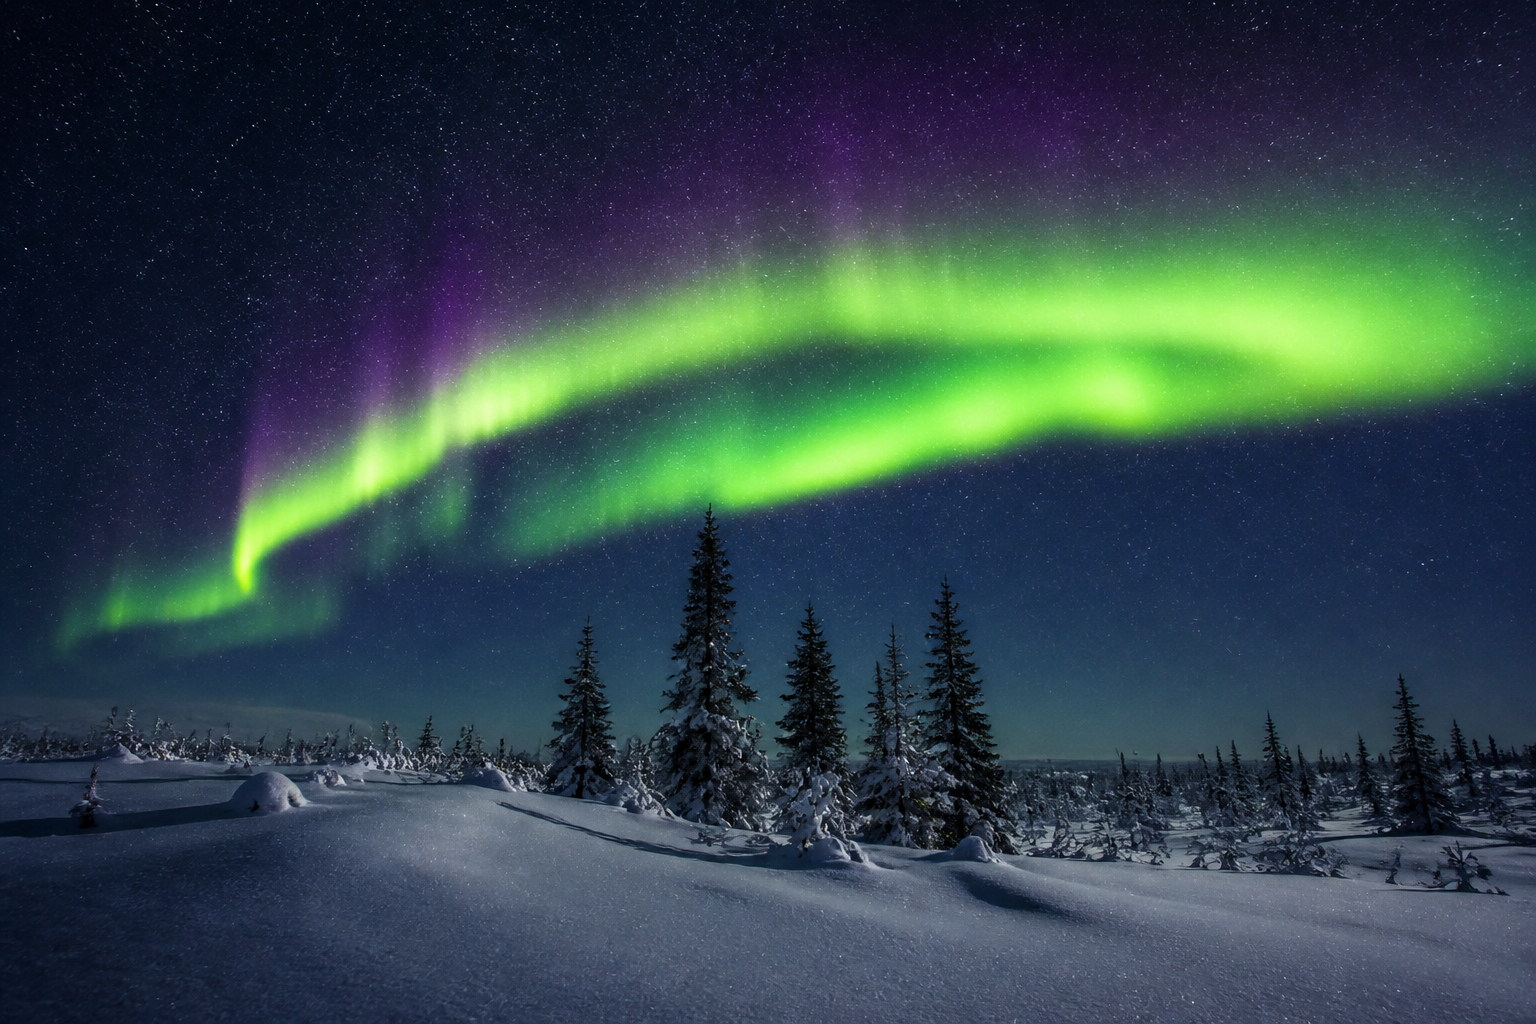
\includegraphics[width=0.58\linewidth]{images/book5/ai/b5-24-aurora-arc.png}

{\small Uma aurora: cargas do vento solar guiadas pelo campo magnético da Terra até a atmosfera polar. O que um observador chama de condução magnética, outro chama de aceleração elétrica --- os campos se misturam sob as transformações deste capítulo.}
\end{omfigure}

\section{Exercícios}

\begin{exercise}[$\star$]\label{exo:b3:covariant-electromagnetism:1}
(a) Aplique a $a^\mu = (5, 3, 0, 0)$ (em unidades de um certo $a_0$) um
impulso de $\beta =
0.6$: calcule $a'^\mu$ e verifique que $a\cdot a$ não muda. (b) Mostre
que a soma de dois \omterm{def:b3:covariant-electromagnetism:fourvector}{quadrivetores} é um \omterm{def:b3:covariant-electromagnetism:fourvector}{quadrivetor}. (c) O $(c,
\vect v)$ de uma partícula é um \omterm{def:b3:covariant-electromagnetism:fourvector}{quadrivetor}? E $\gamma(c, \vect v)$? (d)
Por que ``o campo elétrico'' sozinho não faz parte de \omterm{def:b3:covariant-electromagnetism:fourvector}{quadrivetor} algum?
\end{exercise}

\begin{exercise}[$\star$]\label{exo:b3:covariant-electromagnetism:2}
Um fio de cobre de seção \qty{1.0}{mm^2} conduz \qty{10}{A}; a
densidade de elétrons de condução é $n = \qty{8.5e28}{m^{-3}}$. (a)
Calcule a velocidade de deriva. (b) Escreva $J^\mu$ para o fluido de
elétrons e para a rede. (c) Verifique a equação da continuidade para
cada um. (d) O fio é neutro: quanto vale $J^\mu$ para o fio inteiro, e
que componente sobrevive?
\end{exercise}

\begin{exercise}[$\star$]\label{exo:b3:covariant-electromagnetism:3}
(a) A partir da matriz de $F^{\mu\nu}$, diga que componentes dão
$E_y$ e $B_x$. (b) Escreva $F^{\mu\nu}$ para um campo uniforme puro
$\vect B = B\vect e_z$ e para o campo de uma onda plana
($\vect E = E\vect e_y$, $\vect B = (E/c)\vect e_z$). (c) Verifique nas
componentes que $F^{\mu\nu} = \partial^\mu A^\nu - \partial^\nu
A^\mu$ reproduz $\vect B = \operatorname{\vect{curl}}\vect A$ para
$\mu\nu = 12$. (d) Por que $F$ precisa ser antissimétrico para que a
força $qF^{\mu\nu}u_\nu$ não realize trabalho no referencial próprio da
partícula?
\end{exercise}

\begin{exercise}[$\star$]\label{exo:b3:covariant-electromagnetism:4}
Um capacitor de placas paralelas em repouso mantém
$\vect E = E_0\vect e_y$, sem $\vect B$. Dê $\vect E'$ e $\vect B'$ num
referencial que se move (a) ao longo de $\vect e_y$ (perpendicular às
placas); (b) ao longo de $\vect
e_x$ (paralelo às placas), e interprete o $\vect B'$ que aparece como o
campo das cargas superficiais em movimento; (c) verifique os
invariantes no caso (b); (d) no caso (b), as placas também se contraem:
que grandezas ($\sigma$? $E'$? a separação das placas?) mudam, e de
modo coerente com o quê?
\end{exercise}

\begin{exercise}[$\star\star$]\label{exo:b3:covariant-electromagnetism:5}
A fem de movimento unificada. Uma haste condutora desliza com $\vect v$
sobre trilhos através de um $\vect B$ uniforme. (a) Contabilidade do
laboratório: que força empurra os elétrons ao longo da haste, e que fem
resulta? (b) Contabilidade no referencial da haste: que campo os
empurra, e de onde ele vem na
\cref{prop:b3:covariant-electromagnetism:transform}? (c) Mostre que as
duas fem coincidem em ordem $v/c$. (d) A regra do fluxo de Faraday, do
volume do primeiro ano, cobria tanto o caso ``circuito em movimento''
quanto ``campo variável'' com uma só fórmula: o que a relatividade diz
sobre por que essa unificação tinha de funcionar?
\end{exercise}

\begin{exercise}[$\star\star$]\label{exo:b3:covariant-electromagnetism:6}
(a) Usando a \cref{prop:b3:covariant-electromagnetism:transform},
verifique por cálculo direto que $E'^2 - c^2B'^2 = E^2 - c^2B^2$ para
um impulso ao longo de $x$. (b) Verifique que $\vect E'\cdot\vect B' = \vect
E\cdot\vect B$. (c) Uma região contém $\vect E$ e $\vect B$
perpendiculares, com $E = 2cB$: encontre o referencial de campo
puramente elétrico (direção e velocidade). (d) Por que nenhum
referencial pode tornar o campo de uma onda plana de luz puramente
elétrico ou puramente magnético?
\end{exercise}

\begin{exercise}[$\star\star$]\label{exo:b3:covariant-electromagnetism:7}
Campos cruzados. No laboratório, $\vect E = E\vect e_y$ e $\vect B =
B\vect e_z$ com $E < cB$. (a) Mostre que o referencial que se move com
$\vect v_{\text{d}} = (E/B)\,\vect e_x$ vê um campo puramente
magnético. (b) Descreva o movimento de uma carga solta em repouso,
visto desse referencial e de volta no laboratório (uma cicloide que
deriva a $v_{\text{d}}$). (c) O filtro de velocidades do volume do
primeiro ano deixava passar sem desvio as partículas de velocidade
$E/B$: deduza isso de novo, numa linha, a partir de (a). (d) O que
acontece, qualitativamente, quando $E > cB$ --- e por que o truque do
referencial de deriva se torna então impossível?
\end{exercise}

\begin{exercise}[$\star\star$]\label{exo:b3:covariant-electromagnetism:8}
O \omterm{def:b3:covariant-electromagnetism:fourvector}{quadrivetor} de onda $k^\mu = (\omega/c, \vect k)$. (a) Mostre que
exigir a invariância da fase obriga $k^\mu$ a se transformar como
\omterm{def:b3:covariant-electromagnetism:fourvector}{quadrivetor}. (b) Deduza a fórmula longitudinal do efeito Doppler a
partir de sua componente temporal. (c) Deduza a fórmula da aberração.
(d) Aberração da luz das estrelas: a Terra orbita a \qty{29.8}{km/s};
por que ângulo a posição aparente de uma estrela varre ao longo de um
ano? (Bradley mediu $20.5''$ em 1728 --- a primeira prova direta de que
a Terra se move.)
\end{exercise}

\begin{exercise}[$\star\star$]\label{exo:b3:covariant-electromagnetism:9}
Uma carga $q$ se move com $\vect v = v\vect e_x$ constante, $\gamma \gg
1$. (a) Transformando o campo de Coulomb, mostre que, no plano
transversal que passa pela carga, o campo é amplificado a $\gamma
q/4\pi\varepsilon_0b^2$ à distância $b$, enquanto à frente e atrás ele
é esmagado por $1/\gamma^2$. (b) Mostre que um observador parado à
distância $b$ vê um pulso de campo de duração
$\sim b/\gamma v$. (c) Para um próton do LHC que passa a $b = \qty{1}{cm}$:
campo máximo e duração do pulso. (d) Em que sentido preciso esse pulso
é ``quase luz''? (Verifique $E' \approx cB'$ e os invariantes.)
\end{exercise}

\begin{exercise}[$\star\star\star$]\label{exo:b3:covariant-electromagnetism:10}
Perseguir uma onda de luz. Uma onda plana tem $\vect E = E_0\vect e_y
\cos(\omega(t - x/c))$, $\vect B = (E_0/c)\vect e_z\cos(\omega(t -
x/c))$. Um observador a persegue com $\beta$. (a) Transforme os campos:
mostre que $E'_0 = E_0\sqrt{(1-\beta)/(1+\beta)}$ e $B'_0 = E'_0/c$. (b)
Mostre que a frequência se transforma pelo mesmo fator: a onda continua
onda, desviada para o vermelho, com $E' = cB'$ sempre. (c) O que
acontece com a densidade de energia da onda (proporcional a $E^2$) e
com o número de fótons? (d) Conclua: o que exigiria ``viajar ao lado de
um feixe de luz'', e qual invariante o proíbe?
\end{exercise}

\begin{exercise}[$\star\star\star$]\label{exo:b3:covariant-electromagnetism:11}
A luz síncrotron e a morte das máquinas circulares de elétrons. Uma
carga ultrarrelativística num círculo de raio $r$ irradia a potência
$P = q^2c\gamma^4/6\pi\varepsilon_0r^2$ (admitido --- a fórmula de
Larmor do volume do segundo ano, com o impulso de Lorentz aplicado).
(a) Mostre que a energia perdida por volta é
$\Delta E = q^2\gamma^4/3\varepsilon_0r$. (b) LEP: elétrons a
\qty{100}{GeV} com $r = \qty{3.1}{km}$: calcule $\gamma$ e o
$\Delta E$ por volta --- que fração da energia do feixe é recomprada a
cada volta? (c) LHC: prótons a \qty{6.8}{TeV}, no mesmo túnel: calcule
o $\Delta E$ por volta e compare. (d) Explique, com o fator $\gamma^4 =
(E/mc^2)^4$, por que o sucessor dos elétrons é um colisor
\emph{linear} ou um anel muito maior, e por que os anéis de prótons
sobrevivem.
\end{exercise}

\begin{exercise}[$\star\star\star$]\label{exo:b3:covariant-electromagnetism:12}
O cíclotron relativístico. Uma carga num $\vect B$ uniforme, a
velocidade relativística. (a) A partir de $\dd\vect p/\dd t = q\vect v\wedge\vect
B$ com $E$ constante, mostre que a órbita é um círculo percorrido com
$\omega = qB/\gamma m$: a frequência de cíclotron cai com a energia.
(b) Um cíclotron clássico empurra a $\omega_0 = qB/m$ fixo: mostre que,
após $N$ voltas com $\gamma - 1$ crescendo linearmente até seu valor
final $\Gamma$, o escorregamento de fase acumulado atinge um quarto do
período da radiofrequência quando $\Gamma \approx 1/2N$; para $N = 100$
voltas, que energia cinética de próton é essa, e como ela se compara ao
teto histórico dos cíclotrons clássicos (uns \qty{20}{MeV},
conquistados com margem e tensão extras)? (c) Existem dois remédios:
elevar a frequência (sincrocíclotron) ou moldar $B(r)$ para crescer
como $\gamma$ (cíclotron isócrono): explique cada um numa frase. (d) O
cíclotron isócrono do PSI entrega prótons de \qty{590}{MeV}: por que
fator seu campo na borda supera o campo central?
\end{exercise}

\section{Problema: Magnetismo a passo de caracol}

\begin{problem}[{Problema de fim de semana --- como um desequilíbrio de
$10^{-24}$ faz girar todo motor}]\label{pb:b3:covariant-electromagnetism:1}
Os elétrons derivam por um fio de lâmpada mais devagar que o mel
escorre, e o $v^2/c^2$ dessa deriva vale $10^{-24}$ --- e, ainda assim,
a força magnética que ela produz levanta carros em ferros-velhos. Este
problema faz a contabilidade completa em dois referenciais para um fio
retilíneo e uma carga em movimento, e encontra a relatividade escondida
em todo eletroímã. Dados: fio de cobre, seção $S = \qty{1.0}{mm^2}$,
corrente $I = \qty{10}{A}$, densidade de elétrons de condução
$n = \qty{8.5e28}{m^{-3}}$; carga de prova
$q = \qty{1}{\micro C}$ à distância $d = \qty{1.0}{cm}$, movendo-se
paralelamente ao fio com $v = \qty{e5}{m/s}$ (uma velocidade de feixe
iônico, para manter os números visíveis); $\mu_0 = 4\pi\times10^{-7}\,\unit{H/m}$.

\medskip\noindent\textbf{Parte I --- A contabilidade no laboratório.}
\begin{enumerate}
  \item Calcule a velocidade de deriva $u$ dos elétrons e $u^2/c^2$.
  \item Modele o fio como duas cargas lineares superpostas: a rede
        $+\lambda$ em repouso e os elétrons $-\lambda$ em deriva a
        $u$, com $I = \lambda u$. Calcule $\lambda$.
  \item Calcule $B$ na posição da carga e a força magnética
        $F = qvB$ sobre ela --- direção incluída, para $v$ paralelo à
        corrente convencional $I$ (lembre: correntes paralelas se
        atraem).
  \item Por que não há força \emph{elétrica} alguma no laboratório?
  \item O campo elétrico do mesmo fio se ele carregasse uma carga
        líquida de apenas um elétron em excesso por metro: compare a
        força que ele exerceria sobre $q$ com a força magnética da
        questão 3 e conclua com que precisão a ``neutralidade''
        precisa ser medida antes de o magnetismo poder ser atribuído.
  \item Uma carga de \qty{1}{\micro C} a \qty{e5}{m/s}: a força da
        questão 3 é mensurável? (Compare com o peso de um grão de
        areia, $\sim\qty{e-6}{N}$.)
\end{enumerate}

\medskip\noindent\textbf{Parte II --- Trocando de assento.}
Passe ao referencial da carga de prova (velocidade $v$ ao longo do fio).
\begin{enumerate}[resume]
  \item Nesse referencial, quais são as velocidades da rede e dos
        elétrons (que derivam em sentido oposto a $I$ e por isso
        ganham velocidade neste impulso --- componha-as corretamente)?
  \item Integrada sobre a seção do fio, a quadricorrente por unidade
        de comprimento é $(c\lambda_{\text{tot}}, I, 0, 0)$, com
        $\lambda_{\text{tot}} = 0$ aqui. Transforme-a e mostre que a
        carga linear do fio no novo referencial é
        \[
        \lambda' = -\gamma_v\,\frac{vI}{c^2} .
        \]
  \item Avalie $\lambda'$, em coulombs por metro e em cargas de
        elétron por metro. Qual das duas correntes ficou mais densa, e
        por quê (contraia cada uma separadamente, se preferir)?
  \item Calcule o campo elétrico $E' = \lambda'/2\pi\varepsilon_0d$ na
        carga e a força elétrica $qE'$ sobre ela.
  \item Compare $qE'$ com o $qvB$ do laboratório da Parte I e explique
        o fator residual $\gamma_v \approx 1 + \num{5.6e-8}$ (a lei de
        transformação de qual \omterm{def:b3:covariant-electromagnetism:fourvector}{quadrivetor} relaciona as forças?).
  \item Nesse referencial há também um campo magnético (o fio continua
        conduzindo corrente): por que ele não exerce força aqui?
\end{enumerate}

\medskip\noindent\textbf{Parte III --- A moral dos números.}
\begin{enumerate}[resume]
  \item O desequilíbrio relativo $|\lambda'|/\lambda$: calcule-o e
        escreva-o como $\gamma_v vu/c^2$.
  \item Como um efeito da ordem de $10^{-19}$ da carga do fio pode
        produzir uma força macroscópica? (Que número enorme ele
        multiplica?)
  \item Dois fios paralelos com \qty{10}{A} cada, a \qty{1}{cm}:
        calcule a força por metro e confira contra o valor de
        definição $2 \times 10^{-7}\,I_1I_2/d$ newtons por metro.
  \item Um eletroímã são dez mil voltas desta mesma história: estime o
        campo de uma bobina de \qty{e4}{} espiras por metro conduzindo
        \qty{10}{A} (fórmula do solenoide do volume do primeiro ano) e
        a força por centímetro quadrado que ele exerce sobre o ferro
        ($\sim B^2/2\mu_0$).
  \item Se a relatividade fosse desligada ($c \to \infty$ na
        transformação), o que restaria de $\lambda'$, da força de $B$,
        dos motores e dos ímãs de ferro-velho?
  \item Por que a carga de prova \emph{em repouso} perto do fio não
        sente nada, ainda que os elétrons desfilem ao lado dela? (Que
        cancelamento a protege, e com que exatidão?)
\end{enumerate}

\medskip\noindent\textbf{Parte IV --- Além do fio.}
\begin{enumerate}[resume]
  \item O volume do segundo ano deduzia os campos magnéticos da lei de
        Ampère, com as correntes como fontes dadas. O que este
        capítulo acrescenta a essa contabilidade --- o que \emph{é} o
        campo magnético, visto deste problema?
  \item Os ímãs de ferro não têm bateria: o que faz o papel da
        corrente no magnetismo permanente (uma frase; a resposta
        microscópica honesta é quântica e espera cinco capítulos)?
  \item Um único feixe de elétrons no vácuo (sem rede): um observador
        que o acompanha o vê atrair ou repelir a si mesmo mais do que
        um observador de laboratório? Reconcilie as contabilidades dos
        dois referenciais para a autoconstrição de um feixe.
  \item Torne quantitativo o último ponto: mostre que dois feixes
        paralelos de mesma carga que se movem juntos com $\beta$ se
        repelem com uma força líquida (repulsão elétrica menos atração
        magnética) reduzida exatamente por $1/\gamma^2$ em relação ao
        valor em repouso --- e diga qual contabilidade torna o fator
        evidente.
  \item A energia de uma lâmpada chega a quase $c$, enquanto seus
        elétrons derivam um metro por hora: o que de fato transporta a
        energia ao longo do fio (lembre o vetor de Poynting do volume
        do segundo ano)?
  \item Estime $vu/c^2$ para os elétrons deste problema e uma carga de
        prova de pedestre ($v = \qty{1}{m/s}$): mesmo aí, a força é
        mensurável em primeira ordem com uma agulha de bússola ---
        quem demonstrou que uma corrente desvia uma bússola, e em que
        ano?
  \item Resuma o resultado central: um fio neutro de \qty{10}{A},
        observado de um assento que se move a \qty{e5}{m/s}, carrega
        $-\qty{e-11}{C/m}$ de carga relativística --- e esse erro de
        contabilidade da ordem de $10^{-24}$, devido à \omterm{prop:b3:relativistic-kinematics:contraction}{contração dos
        comprimentos}, multiplicado por $10^{28}$ elétrons, é a força
        magnética inteira do laboratório.
\end{enumerate}
\end{problem}
